\section{The Queue Transmission Model}


%% TODO(fwt): We need to say that we handle expected number of cars instead of
%% physical cars, so its fine to have fractions of cars.

A Queue Transmission Model (QTM) is the tuple $(\Qset, \Lset, \vecDT, \MatQIN)$,
where \Qset and \Lset are, respectively, the set of queues and lights;
%
\vecDT is a vector of size \Nn representing the discretization of the simulation
horizon $[0,\TMAX]$ and the duration in seconds of the $n$-th time interval is
denoted as \DT[n];
%
%%
%% TODO(fwt): Maybe mention that car that are denied entry could be stored in a
%% infinity capacity queue and eventually be allowed to enter the network. Also
%% point out that this case doesn't happen in our experiments
%%
%% TODO(fwt): Maybe mention that add \QIN{i} can estimate through a model
%% learned from historical data.
%
and \MatQIN is a matrix $|\Qset| \times \TMAX$ in which \QIN{i}{n} represents
the flow of cars requesting to enter queue $i$ from the outside of the network
at time $n$.



A \textbf{traffic light} $\tl \in \Lset$ is defined as the tuple~$(\CTMIN{\tl},
\CTMAX{\tl}, \Pset_\tl, \VecPTMIN{\tl}, \VecPTMAX{\tl})$, where:

\begin{itemize}
%
\item $\Pset_\tl$ is the set of phases of $\tl$;
%
\item \CTMIN{\tl} (\CTMAX{\tl}) is the minimum (maximum) allowed cycle time for
  \tl; and
%
\item \VecPTMIN{\tl} (\VecPTMAX{\tl}) is a vector of size $|\Pset_\tl|$ and
  \PTMIN{\tl}{k} (\PTMAX{\tl}{k}) is the minimum (maximum) allowed time for
  phase $k \in \Pset_\tl$. 
%
\end{itemize}


A \textbf{queue} $i \in \Qset$ represents a segment of road that vehicles
traverse at free flow speed; once traversed, the vehicles are vertically stacked
in a stop line queue.
% of maximum capacity \QMAX{i}.
%
Formally, a queue~$i$ is defined by the tuple~$(\QMAX{i}, \QDELAY{i}, \QOUT{i},
\Fvec_i, \Prvec_i, \QPset{i})$ where:

\begin{itemize}
%
%% TODO(fwt): clarify that this is the capacity of stop line queue
\item \QMAX{i} is the maximum capacity of $i$;
%
\item \QDELAY{i} is the time required to traverse $i$ and reach the stop line;
%
\item \QOUT{i} represents the maximum traffic flow from $i$ to the outside of
  the modeled network;
%
\item $\Fvec_i$ and $\Prvec_i$ are vectors of size \Qn and their $j$-th entry
  (i.e., \FMAX{i}{j} and \FTURN{i}{j}) represent the maximum flow from queue $i$
  to $j$ and the turn probability from $i$ to $j$ ($\sum_{j \in
  \Qset}\FTURN{i}{j} = 1$), respectively; and
%
\item \QPset{i} denotes the set of traffic light phases controlling the outflow
  of queue $i$.
%
\end{itemize}


Differently than CTM \cite{daganzo1994cell,lin2004enhanced}, QTM does not assume
that \remark{$\DT[n] = \QDELAY{i}$} for all \mbox{$n \in \{1,\dots,\Nn\}$}, that
is, the QTM can represent non-homogeneous time intervals.
%
The only requirement over \DT[n] is that no traffic light maximum phase time is
smaller than any \DT[n] since phase changes occur only between time intervals;
formally, $\DT[n] \le \min_{\tl \in \Lset, k \in \Pset_\tl} \PTMAX{\tl}{k}$ for
all $n \in \{1,\dots,\Nn\}$.
%
\toIain{Maybe bring forward a small network and any other figure that would help
illustrate the model and comment about it.}




\subsection{Traffic Flow Simulation with QTM}\label{sec:lp}

In this section, we present how to simulate traffic flow in a network using QTM
and non-homogeneous time intervals \DT[].
%
We assume for the remainder of this section that a \emph{valid} control plan for
all traffic lights is fixed and given as parameter;
%
formally, for all $\tl \in \Lset$, $k \in \Pset_\tl$, and interval $n \in
\{1,\dots,N\}$, the binary variable $\p{\tl}{k}$ is known a priori and indicates
if phase $k$ of light \tl is active~(i.e., $\p{\tl}{k} = 1$) or not on interval
$n$.


We represent the problem of finding the flow between queues as a Linear Program
(LP) over the following variables defined for all interval $n \in
\{1,\dots,\Nn\}$ and queues $i$ and $j$:

\begin{itemize}
%
\item $\q{i} \in [0,\QMAX{i}]$: traffic volume of queue $i$ during interval $n$;
%
\item $\inq{i} \in [0,\QIN{i}{n}]$: inflow to the network via queue $i$
during interval $n$;
%
\item $\outq{i} \in [0,\QOUT{i}]$: outflow from the network via queue $i$ during
interval $n$; and
%
\item $\f{i}{j} \in [0,\FMAX{i}{j}]$: flow from queue $i$ into queue $j$ during
interval $n$.
%
\end{itemize}

%% FWT: These constraints are not necessary because we defined the domain of the
%% variables in the paragraph above
%\inq{i} &\le \QIN{i}{n} \tag{C1}\label{eq:C1}\\ 
%\outq{i} &\le \QOUT{i} \tag{C2}\label{eq:C2}\\
% \q{i} &\le \QMAX{i} \tag{C9}\label{eq:C9}\\


The maximum traffic flow from queue $i$ to queue $j$ is enforced by
\cref{c:turnProb,c:maxFlow}.
%
\eqref{c:turnProb} ensures that only the fraction $\FTURN{i}{j}$ of the total
internal outflow of $i$ goes to $j$, and \eqref{c:maxFlow} forces the flow from
$i$ to $j$ to be zero if all phases controlling $i$ are inactive (i.e.,
$\p{\ell}{k} = 0$ for all $k \in \QPset{i}$).
%
If more than one phase $\p{\ell}{k}$ is active, then \eqref{c:maxFlow} is
subsumed by the domain upper bound of $\f{i}{j}$.
%
\begin{cAlign}
\f{i}{j} &\le \FTURN{i}{j} \sum_{k=1}^{\Qn}  \f{i}{k} \tagconstrain{c:turnProb}\\
\f{i}{j} &\le \FMAX{i}{j} \sum_{\p{\ell}{k} \in \QPset{i}} {\p{\ell}{k}}
\tagconstrain{c:maxFlow}
\end{cAlign}


%% TODO(fwt): improve the beginning of this paragraph

To simplify the presentation of remainder of the LP, we define the helper
variables \qin{i}~\eqref{def:qin}, \qout{i}~\eqref{def:qout}, and
\tn[n]~\eqref{def:tn} to represent the volume of traffic to enter and leave
queue $i$ during interval~$n$, and the time elapsed since the beginning of the
simulation until the end of interval \DT[n].
%
Using these helper variables, the flow conservation principle for queue $i$ and
\textit{homogeneous} \DT[] is simply $\q{i} = \q[n-1]{i} - \qout[n-1]{i} +
\qin[n-1]{i}$; however, a more sophisticated principle is need for
non-homogeneous time intervals \remark{because \DT[n-1] might be smaller than
\QDELAY{i}, therefore, there are cars at the stop line of $i$ in the beginning
of \DT[n] that started traversing $i$ before \DT[n-1].}
%
\toIain{Triple check my explanation.}
%
%% FWT: Text related to the removed constraint:
%with the constraint \ref{eq:C7} that the total flow out of queue $i$ during
%interval $n$ cannot exceed the sum of the volume of the queue at the start of
%that interval and the volume of traffic arriving at the stop line during the
%interval.
%
\begin{cAlign}
%
\qin{i} &= \DT (\inq{i} + \sum_{j=1}^{\Qn} \f{j}{i}) \tagconstrain{def:qin} \\
%
\qout{i} &= \DT (\outq{i} +  \sum_{j=1}^{\Qn} \f{i}{j})
\tagconstrain{def:qout}\\
%
\tn[n] &= \sum_{x=1}^{n} \DT[x] \tagconstrain{def:tn}
%
\end{cAlign}
\toFelipe{Do we really need this as a constraint?}

In order to account for the \remark{misalignment} of the different \DT[] and
\QDELAY{i}, we need to find the volume of traffic that was able to arrive at
queue $i$, traverse it (i.e., wait \QDELAY{i} seconds), and reach the stop line
before \DT[n] is over.
%
%% TODO(fwt): improve this explanation
%
This volume of traffic is obtained by integrating over the current interval
with the rate at which traffic was arriving during the interval $m$ containing
the time $\tn - \QDELAY{i}$, where $m$ is the interval such that $\tn[m] \le
\tn-\QDELAY{i} < \tn[m+1]$.
%
The input rate of queue $i$ during interval $m$ is found by dividing
$\qin[m]{i}$ with $\DT[m]$, and then the total traffic arriving during the
interval $n$ is found by multiplying this rate by $\DT$.
%
The flow conservation principle for non-homogeneous time steps is presented in
\eqref{c:qUpdate}.
%
To insure that the total volume of traffic travelling down the queue and waiting
at the stop line does not exceed the capacity if the queue, we apply
\eqref{c:10}.
%
\begin{cAlign}
%
\q{i} &= \q[n-1]{i} - \qout[n-1]{i} + \frac{\DT[n]}{\DT[m]}\qin[m]{i}
\tagconstrain{c:qUpdate}\\
%
\frac{\DT[n]}{\DT[m]}\qin[m]{i}  + \sum \limits_{k=m+1}^n \qin[k]{i} &\le
\QMAX{i} - \q[n-1]{i} \tagconstrain{c:10}
%
\end{cAlign}


\remark{Show diagrams with traffic predictions converging as time increment gets
smaller.  Validates that large time-steps are rough approximations while model
behavior converges for small time steps.}

\begin{figure*}[t!]
\centering
%  trim={<left> <lower> <right> <upper>}
\subfigure[]{
\label{subfig:converg_a}
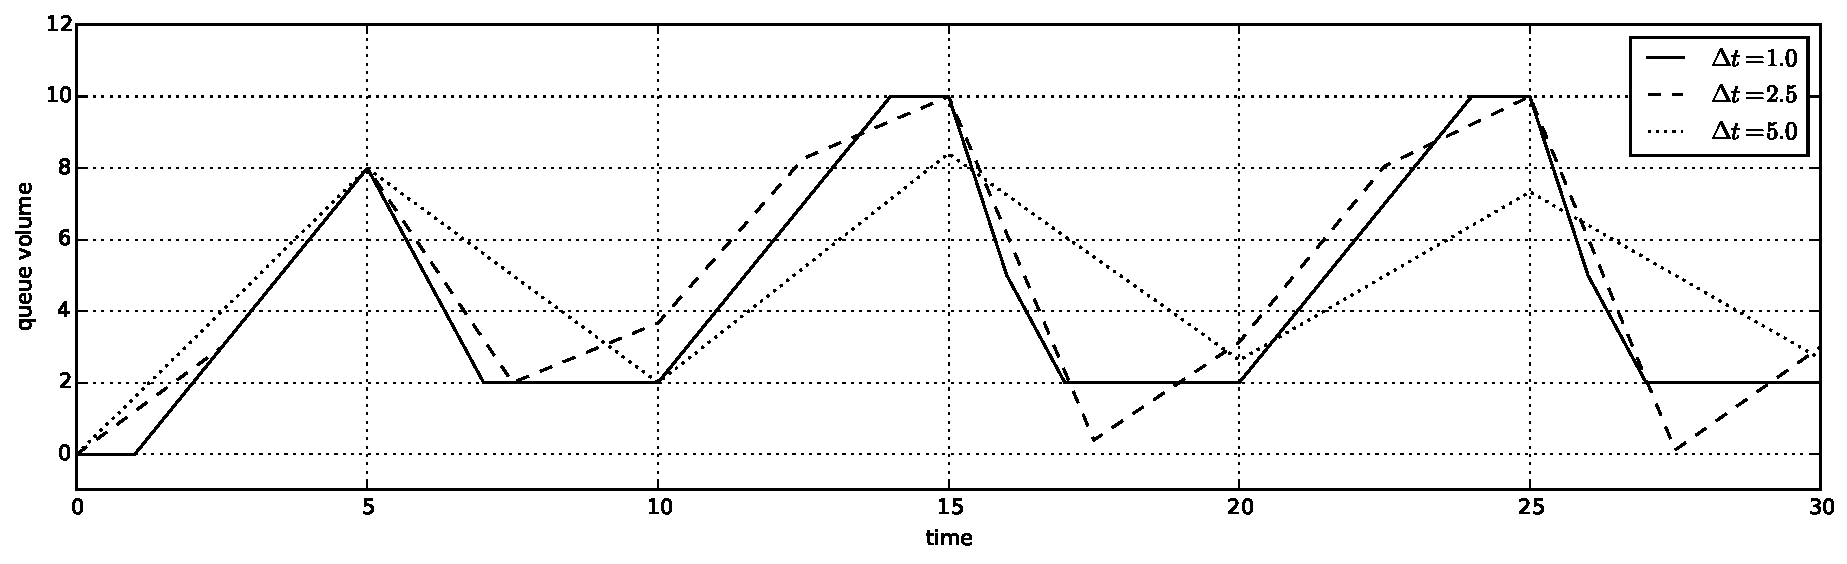
\includegraphics[width=1.0\textwidth,trim={0cm 0cm 0cm 0cm},clip]{convergence.pdf}
}
\subfigure[]{
\label{subfig:converg_b}
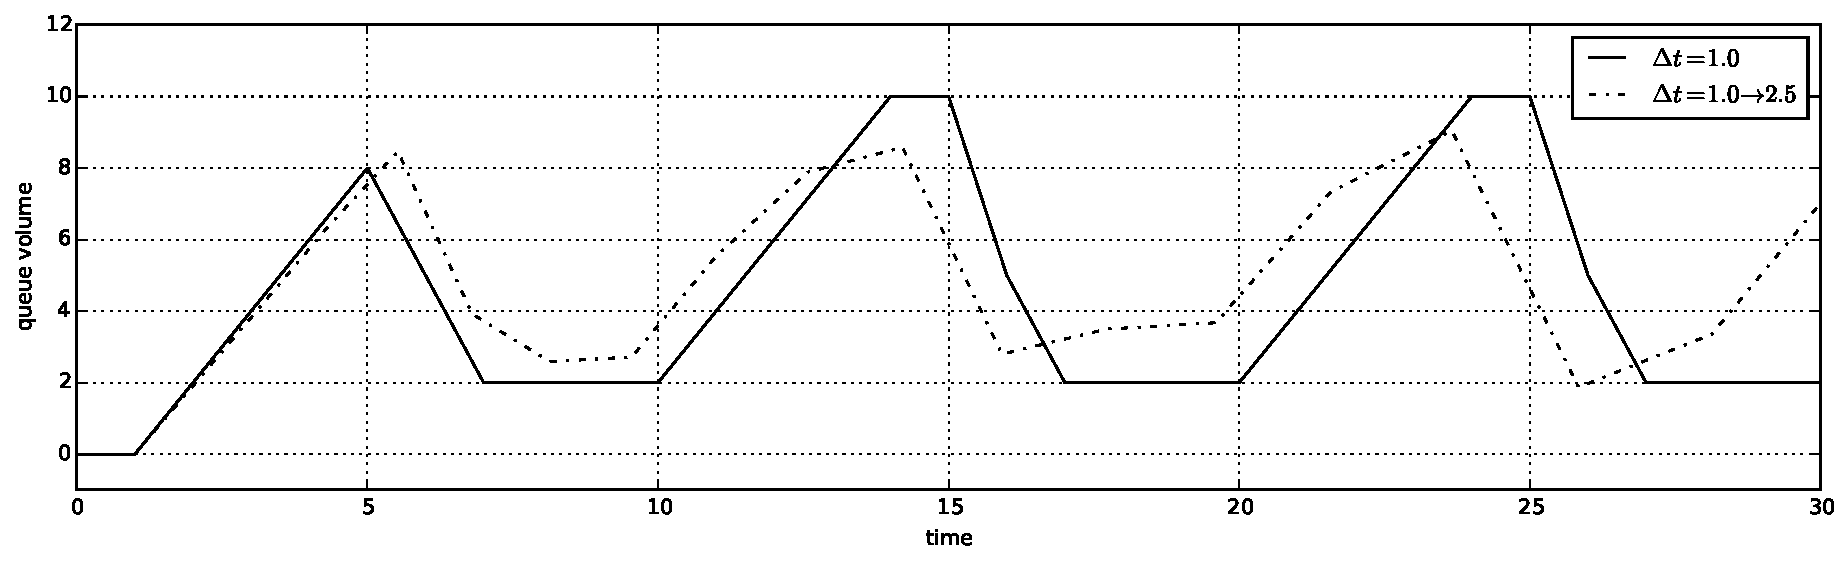
\includegraphics[width=1.0\textwidth,trim={0cm 0cm 0cm 0cm},clip]{convergence_vari.pdf}
}
\caption{An example showing the evolution of traffic volume in a queue over
time. (a) Convergce with increasing refinement of $\Delta t$ from $5.0$ down to
$1.0$. (b) Dilation of $\Delta t$ from $1.0$ to $2.5$ compared to a fixed
$\Delta t$ of $1.0$.}

\end{figure*}

\begin{figure*}[t!]
\centering
%  trim={<left> <lower> <right> <upper>}

\label{subfig:converg_c}
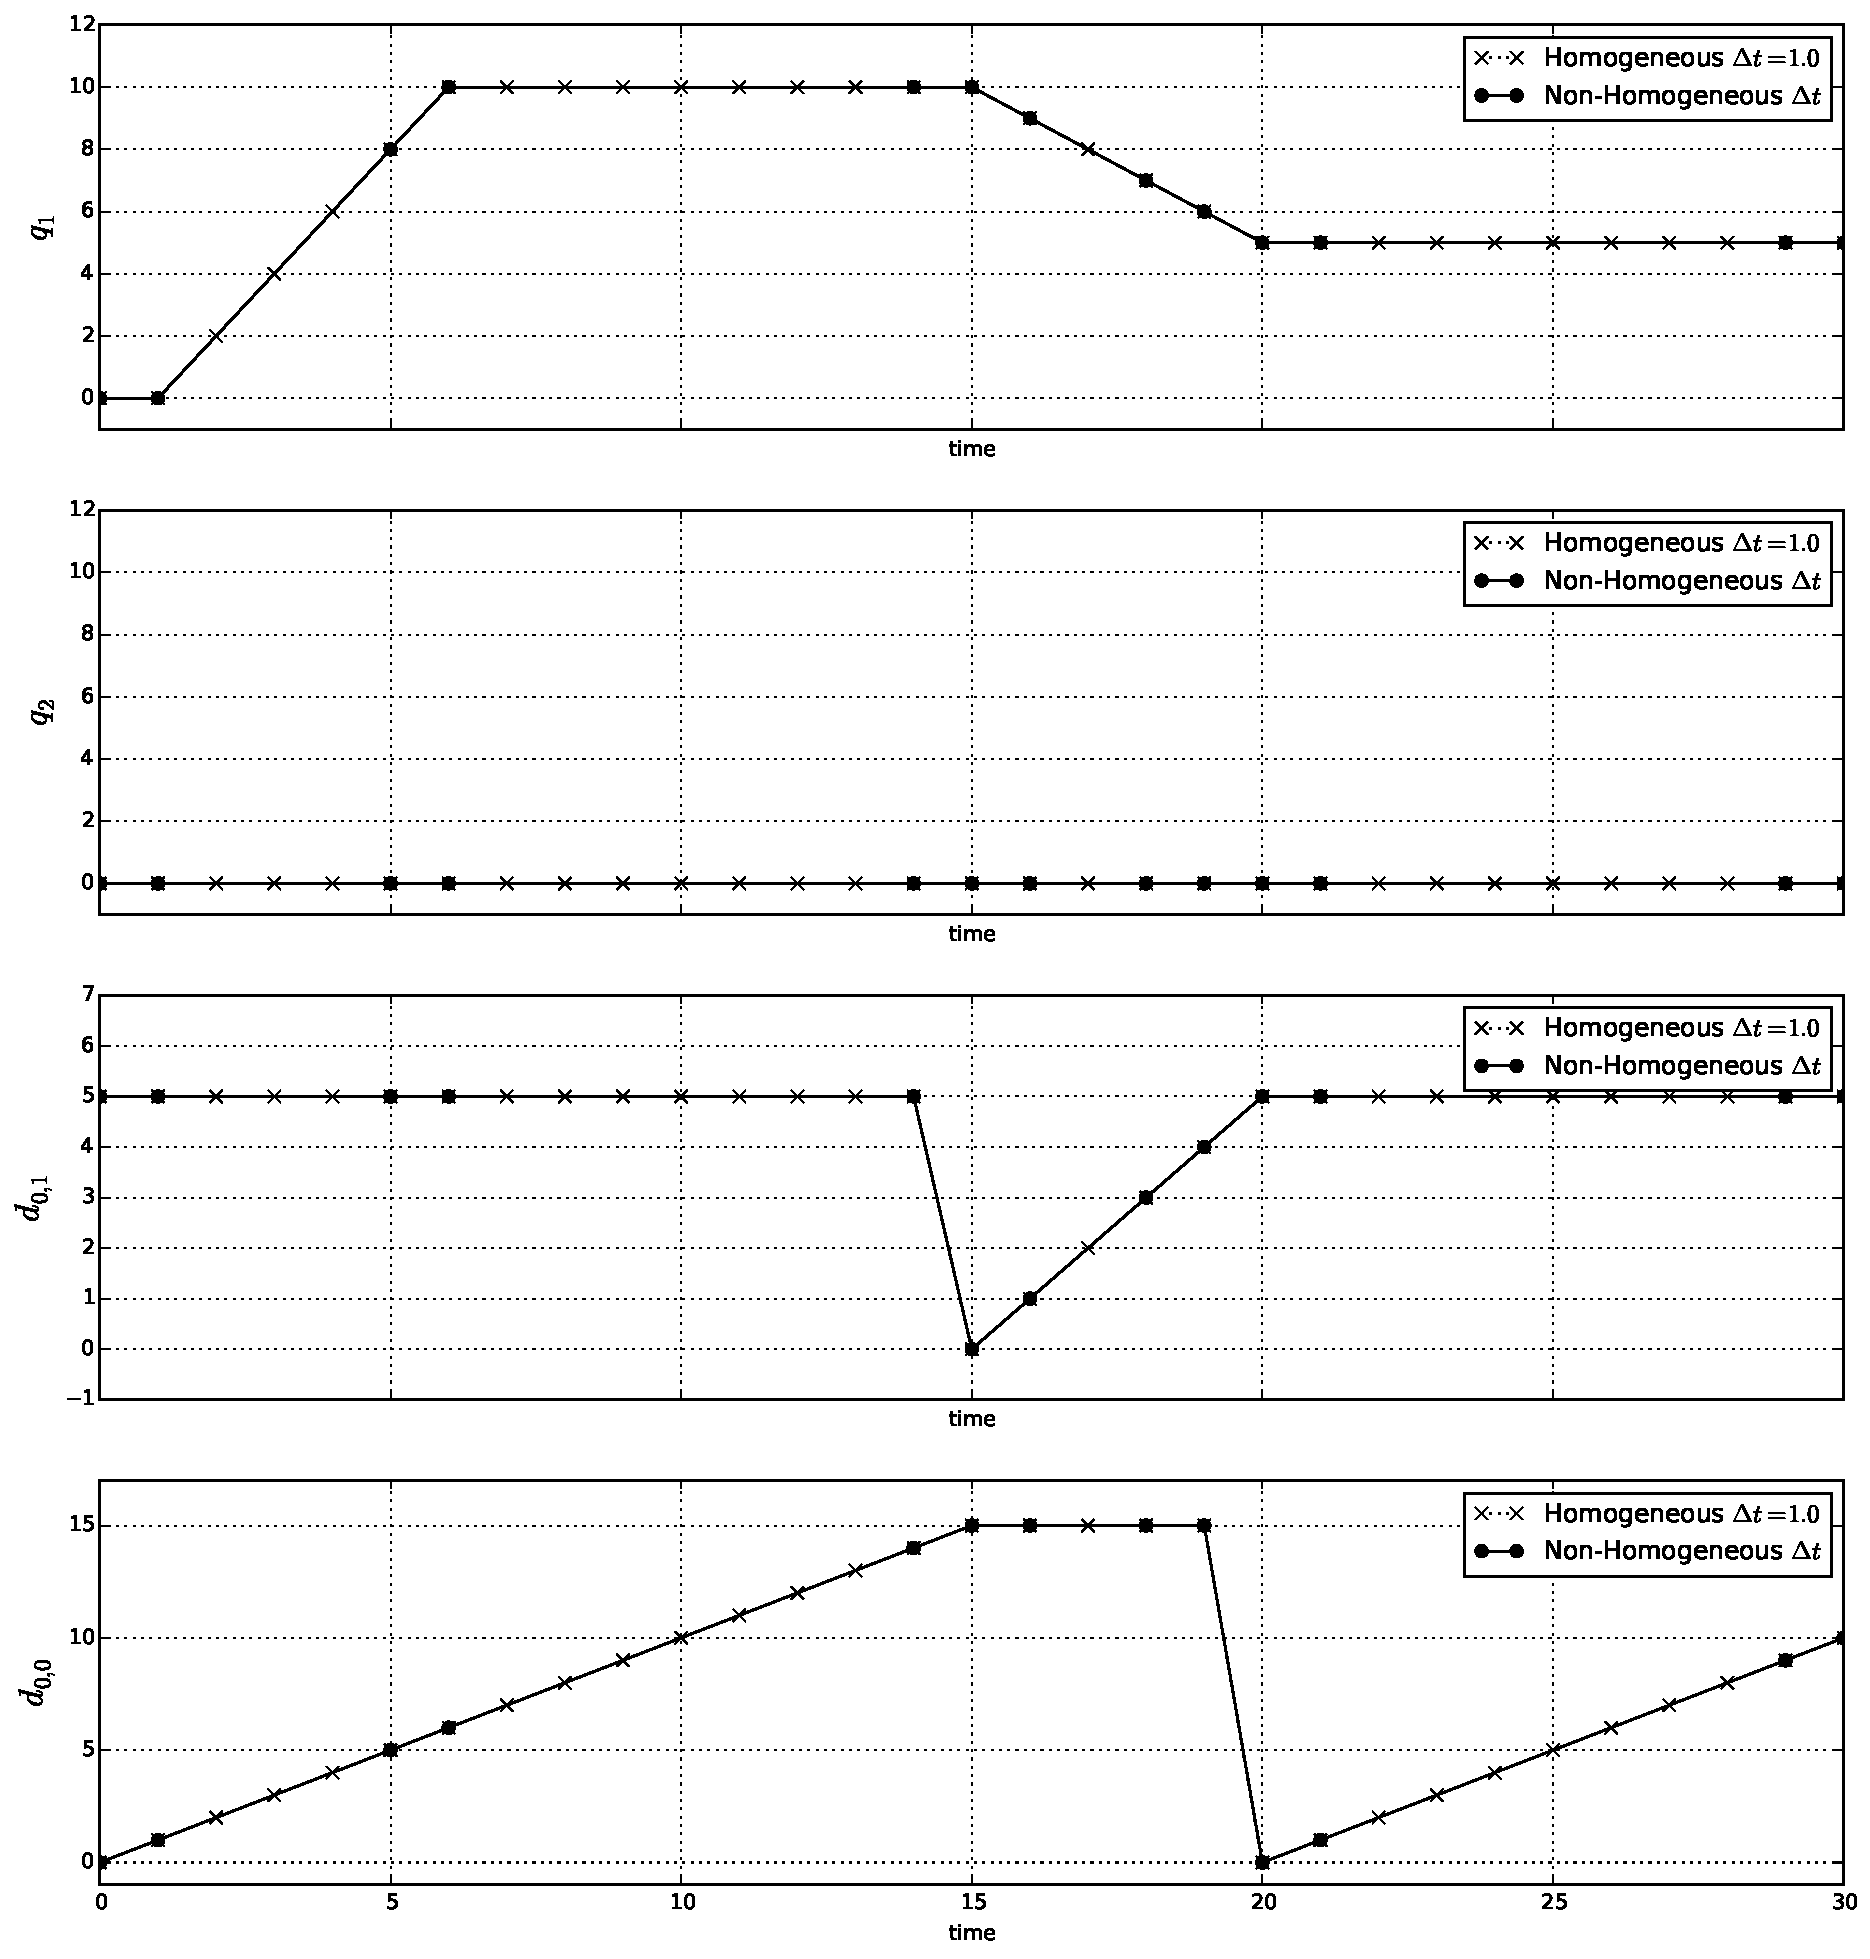
\includegraphics[width=1.0\textwidth,trim={0cm 0cm 0cm 0cm},clip]{convergence_NH.pdf}
\caption{An example showing the convergence between a homogeneous solution with
$\Delta t=1.0$ and a non-homogeneous solution over 30 seconds for the same
network. By using non-homogeneous time steps the same solution is found with
only 14 sample points compared to 30 for homogeneous solution.}

\end{figure*}



As CTM, QTM is also susceptible to \emph{withholding traffic}, i.e., the
optimizer might prevent cars from moving from $i$ to $j$ even though the
associated traffic phase is active and $j$ is not full.
%
We address this issue through our objective function~\eqref{eq:objFunc} by
maximizing the total outflow~\qout{i}~(i.e., both internal and external outflow)
of~$i$ plus the inflow~\inq{i} from the outside of the network to~$i$.
%
This quantity is weighted by the remaining time until the end of the simulation
horizon \TMAX to force the optimizer to allow as much traffic volume as possible
into the network and move traffic to the outside the network as soon as
possible.
%
\eqref{eq:objFunc} is \remark{analogous} to minimizing delay in CTM models,
e.g., \eqref{eq:objFunc} is equivalent to the objective function (O3) in
\trbcite{lin2004enhanced} for their parameters $\alpha = \beta = 1$. \toIain{Add
a paragraph linking the plots with the objective function.}

%% FWT: not sure if we need to give this extra details
%\trbcite{lin2004enhanced} derive an objective function for the minimisation of
%total delay based on the difference between the cumulative departure and
%arrival curves at the origin and destination. However, such an approach
%requires the network to be cleared at the end of the optimisation period.


\begin{equation}
\max 
 \sum_{n=1}^{\Nn} \sum_{i=1}^{\Qn} (\TMAX - \tn + 1) (\qout{i} + \inq{i})
\tag{O1}\label{eq:objFunc}
\end{equation}


The objective function~\eqref{eq:objFunc} and
constraints~(\ref{c:turnProb}--\ref{c:10}) form the LP representing the
dynamic, piecewise linear model of flow in a QTM network over time when a
control plan \p{\tl}{k} is given as an input parameter.



\section{Traffic Control with QTM as an MILP}

In this section, we remove the assumption that a valid control plan for all
traffic lights is given and extend the LP
(\ref{eq:objFunc},~\ref{c:turnProb}--\ref{c:10}) to an Mixed-Integer LP (MILP)
that also computes the optimal control plan.
%
Formally, for all~$\tl \in \Lset$, $k \in \Pset_\tl$, and interval $n \in
\{1,\dots,N\}$, the phase activation parameter~$\p{\tl}{k} \in \{0,1\}$ becomes
a free variable to be optimized.
%
In order to obtain a valid control plan, we enforce that one phase of traffic
light \tl is always active at any interval~$n$~\eqref{c:onlyOnePhaseOn} and that
phase changes happen sequentially~\eqref{c:seqPhases}, i.e., if phase~$k$ was
active during interval~$n-1$ and has become inactive in interval~$n$, then
phase~$k+1$ must be active in interval~$n$.
%
\eqref{c:seqPhases} assumes that $k+1$ equals 1 if $k = \Pn{}$.
%
\toIain{I removed the constraint $\p{\ell}{k} + \p{\ell}{k+1} \le 1$ because it
is subsumed by $\p{\ell}{k} \in \{0,1\}$ and \eqref{c:onlyOnePhaseOn}}


%% FWT: note sure if the text bellow is necessary
%Note that there could be more than one queue mapped to each $\p[]{\ell}{k}$, or
%their could be none

\begin{cAlign}
%
\sum\limits_{k=1}^{\Pn} \p{\ell}{k} &= 1\tagconstrain{c:onlyOnePhaseOn}\\
%
\p[n-1]{\ell}{k} &\le \p{\ell}{k} + \p{\ell}{k+1}\tagconstrain{c:seqPhases}
%
\end{cAlign}


Next, we enforce the minimum and maximum phase durations (i.e.,
$\PTMIN{\ell}{k}$ and $\PTMAX{\ell}{k}$) for each phase $k \in \Pset_\tl$ of
traffic light \tl.
%
To encode these constraints, we use the helper variable $\pd{\ell}{k} \in
[0,\PTMAX{\ell}{k}]$ defined by constraints (\ref{c:pd:incUB}--\ref{c:pd:reset})
that:
%
(i) holds the elapsed time since the start of phase $k$ when $\p[n]{\ell}{k}$ is
active~(\ref{c:pd:incUB},\ref{c:pd:incLB});
%
(ii) is constant and holds the duration of the last phase until the next
activation when $\p[n]{\ell}{k}$ is
inactive~(\ref{c:pd:inactiveUB},\ref{c:pd:inactiveLB}); and
%
(iii) is restarted when phase~$k$ changes from inactive to
active~\eqref{c:pd:reset}.
%
Notice that (\ref{c:pd:incUB}--\ref{c:pd:reset}) employs the \textit{big-M}
method to turn the cases that should not be active into subsumed constraints
based on the value of $\p[]{\tl}{k}$.
%
We use~\PTMAX{\ell}{k} as our large constant since $\pd[n]{\ell}{k} \le
\PTMAX{\ell}{k}$ and $\DT[n] \le \PTMAX{\ell}{k}$ by assumption (\cref{sec:lp}).
%
Similarly, \cref{c:minPhase} ensures the minimum phase time of $k$ and is
not enforced while $k$ is still active.
%
%% FWT: I think the mathematical definition of \pd is redundant now.
%\begin{equation}
%\pd{\ell}{k} = 
%\begin{cases}
%\pd[n-1]{\ell}{k} + \DT[n-1] & \p[n-1]{\ell}{k}=1,\p{\ell}{k}=1\\
%\pd[n-1]{\ell}{k} & \p{\ell}{k}=0\\
%0 & \p[n-1]{\ell}{k}=0,\p{\ell}{k}=1
%\end{cases}
%\label{def:pd}
%\end{equation}
%
%% TODO(fwt): I believe that that \pd{\ell}{k} (above) could be redefined by
%% shifting it by delta_n resulting in a d_{l,k,n} representing the total time
%% until the end of interval **n** instead of n-1. This would be more intuitive
%% and would simplify c:cycleLB and c:cycleUB. This is what I propose:
%% d_{l,k,n} = d_{l,k,n-1} + delta-t_{n}  if p_{l,k,n-1} = p_{l,k,n} = 1
%%           = d_{l,k,n-1}                if p_{l,k,n} = 0
%%           = delta-t_{n}                if p_{l,k,n-1} 0 and p_{l,k,n} = 1
%
%% FWT: this constraint is define as the variable domain
%\pd{\ell}{k} &\le \PTMAX{\ell}{k}\tag{C19}\label{eq:C19}\\
%
\begin{cAlign}
%
\pd{\ell}{k} &\le
  \pd[n-1]{\ell}{k} + \DT[n-1] \p[n-1]{\ell}{k} 
  + \PTMAX{\ell}{k} (1 - \p[n-1]{\ell}{k})\tagconstrain{c:pd:incUB}\\
%
\pd{\ell}{k} &\ge
  \pd[n-1]{\ell}{k} + \DT[n-1] \p[n-1]{\ell}{k}
  - \PTMAX{\ell}{k} (1 - \p[n-1]{\ell}{k})\tagconstrain{c:pd:incLB}\\
%
\pd{\ell}{k} &\le \pd[n-1]{\ell}{k} + \PTMAX{\ell}{k} \p[n-1]{\ell}{k}
  \tagconstrain{c:pd:inactiveUB}\\
%
\pd{\ell}{k} &\ge \pd[n-1]{\ell}{k} - \PTMAX{\ell}{k} \p{\ell}{k}
  \tagconstrain{c:pd:inactiveLB}\\
%
\pd{\ell}{k} &\le \PTMAX{\ell}{k}(1 - \p{\ell}{k} + \p[n-1]{\ell}{k})
  \tagconstrain{c:pd:reset}\\
%
\pd{\ell}{k} &\ge \PTMIN{\ell}{k}(1 - \p{\ell}{k}) \tagconstrain{c:minPhase}
\end{cAlign}



Finally, we constrain the sum of all the phase durations for light \tl to be
within the cycle time limits \CTMIN{\tl}~\eqref{c:cycleLB} and
\CTMAX{\tl}~\eqref{c:cycleUB}.
%
In both \eqref{c:cycleLB} and \eqref{c:cycleUB}, we use the duration of phase 1
of \tl from the previous interval $n-1$ instead of the current interval $n$
because \eqref{c:pd:reset} forces \pd[n]{\tl}{1} to be 0 at the beginning of
each cycle;
%
however, from the previous end of phase 1 until $n-1$, \pd[n-1]{\tl}{1} holds
the correct elapse time of phase 1.
%
Additionally, \eqref{c:cycleLB} is enforced right after the end of the each
cycle, i.e., when its first phase is changed from inactive to active.
%
\toIain{Relate the phase and cycle constraints with the plots}
%
\begin{cAlign}
%
\pd[n-1]{\ell}{1} + \sum\limits_{k=2}^{\Pn} \pd{\ell}{k} &\ge \CTMIN{\ell}
(\p{k}{1} - \p[n-1]{k}{1}) \tagconstrain{c:cycleLB}\\
%
\pd[n-1]{\ell}{1} + \sum\limits_{k=2}^{\Pn} \pd{\ell}{k} &\le \CTMAX{\ell}
\tagconstrain{c:cycleUB}
%
\end{cAlign}


\remark{Extend the conclusion of this section}

The MILP that encodes the problem of finding the optimal traffic control plan in
a QTM network is defined
by~(\ref{eq:objFunc},~\ref{c:turnProb}--\ref{c:cycleUB}).



\begin{figure*}[t!]
\centering
%  trim={<left> <lower> <right> <upper>}
\subfigure[]{
\label{subfig:test1}
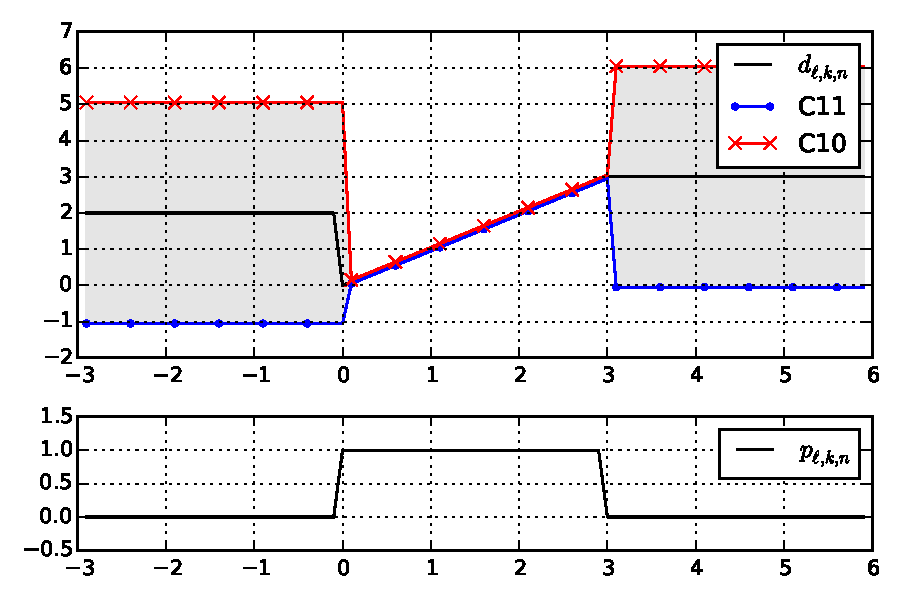
\includegraphics[width=0.45\textwidth,trim={0cm 0cm 0cm 0cm},clip]{phase_plot_fig_1.pdf}}
\subfigure[]{
\label{subfig:test2}
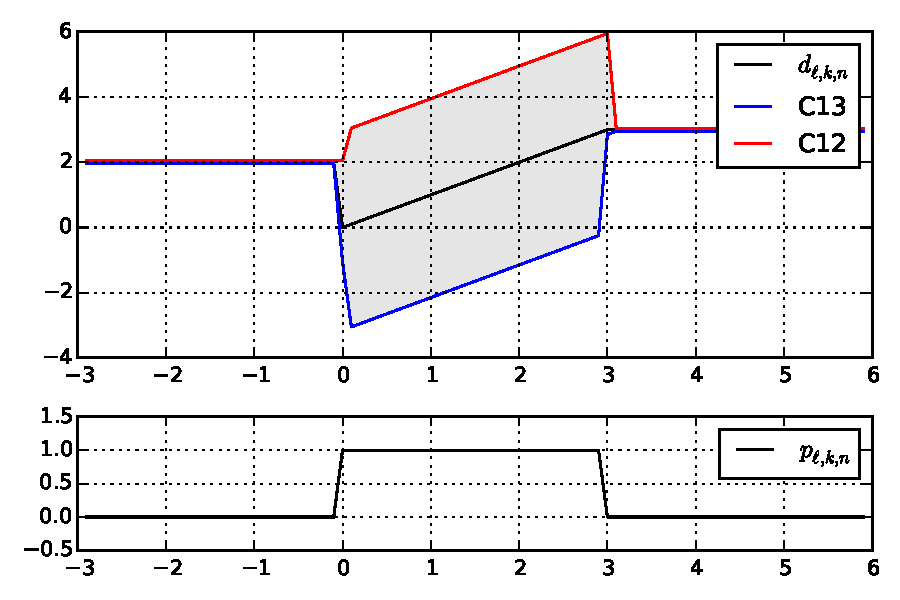
\includegraphics[width=0.45\textwidth,trim={0cm 0cm 0cm 0cm},clip]{phase_plot_fig_2.pdf}}
\subfigure[]{
\label{subfig:test3}
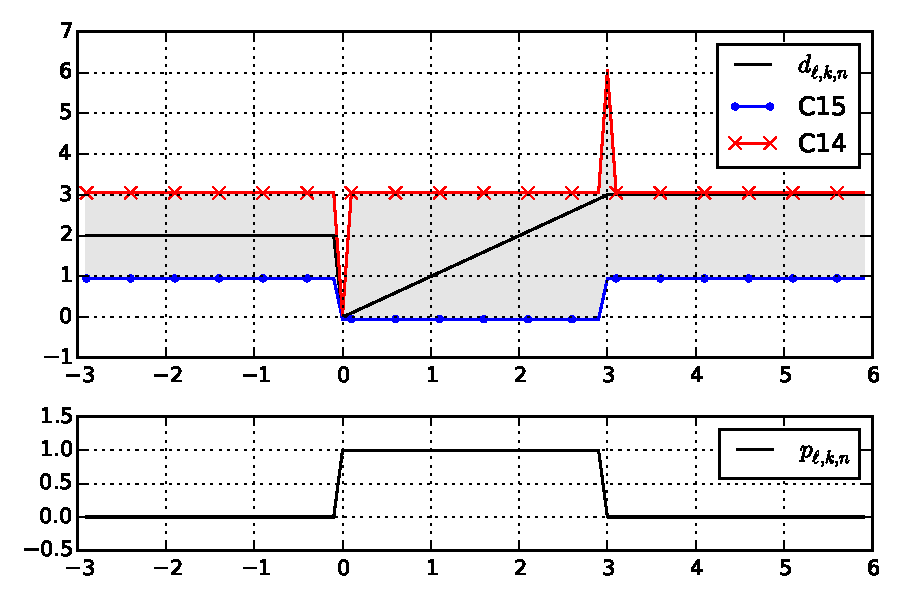
\includegraphics[width=0.45\textwidth,trim={0cm 0cm 0cm 0cm},clip]{phase_plot_fig_3.pdf}}
\subfigure[]{
\label{subfig:test4}
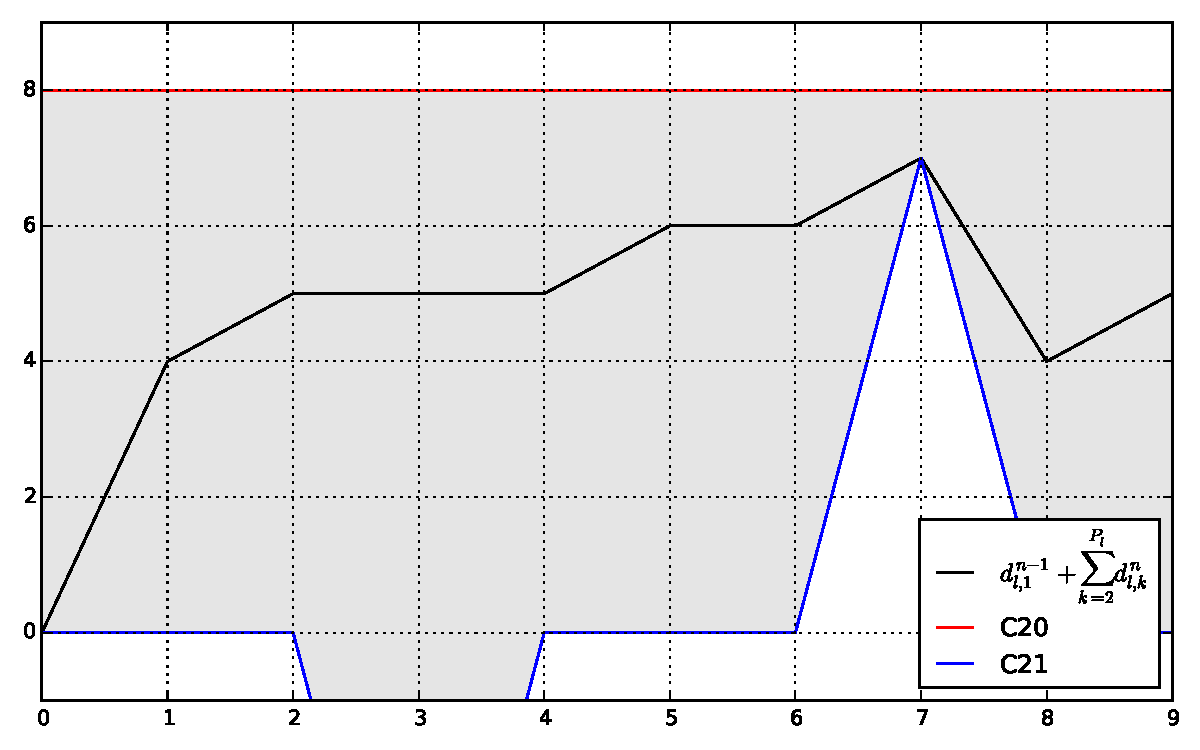
\includegraphics[width=0.45\textwidth,trim={0cm 0cm 0cm 0cm},clip]{phase_plot_fig_4.pdf}}
\caption{An example showing the phase and cycle time constraint envelopes. In
(a), (b) and (c), $\PTMIN{\ell}{k}=1$ and $\PTMAX{\ell}{k}=3$, the duration of
the previous activation was 2 and the duration of the current activation is 3.
In (d), the total cycle time is 7 with $\CTMIN{\ell}=7$, $\CTMAX{\ell}=8$}
\label{fig:phase_plots}
\end{figure*}

